\paragraph{Legge di Young-Laplace.}
\begin{minipage}{0.60\textwidth}
La superficie di interfaccia tra due liquidi può essere modellata come una membrana, una superficie bidimensionale all'interno della quale agisce una forza per unità di lunghezza, tangente alla superficie stessa. La forza per unità di spessore $\gamma$ agente nella membrana viene definità \textit{tensione superificiale}. La legge di Young-Laplace lega la tensione superficiale, il salto di pressione attraverso la superficie di interfaccia e la curvatura della superficie stessa. Nel caso di tensione superficiale costante, vale
\begin{equation}
  p_b - p_a = \gamma \displaystyle\left( \frac{1}{R_1} + \frac{1}{R_2} \right) = 2 \gamma H
\end{equation}
 dove con $R_1$ e $R_2$ sono stati indicati i due raggi di curvatura della superficie e con $H$ si è indicata la curvatura media.
\end{minipage}
%
\begin{minipage}{0.40\textwidth}
  \begin{center}
    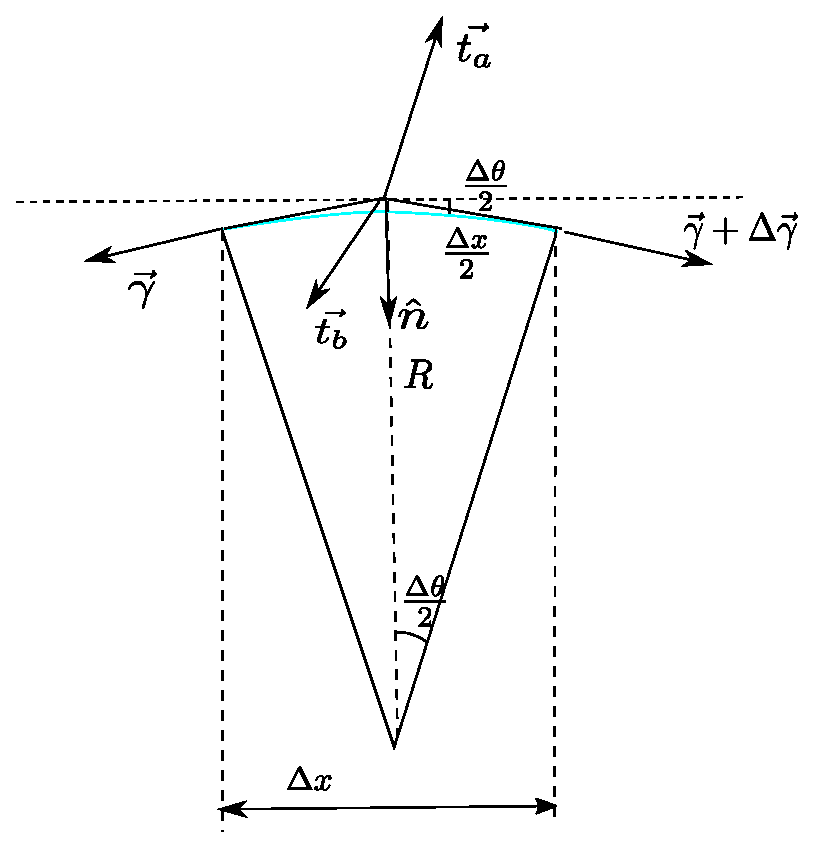
\includegraphics[width=0.95\textwidth]{./fig/laplaceYoung2Ddim.eps}
  \end{center}
\end{minipage}

\paragraph{Legge di Young-Laplace in due dimensioni.}
Viene ricavata la legge di Young-Laplace in due dimensioni, scrivendo l'equilibrio di un elemento di membrana (monodimensionale) soggetta agli sforzi esercitati dai due fluidi su di essa e alla tensione superficiale al suo interno. L'equazione vettoriale di equilibrio viene proiettata in direzione normale e tangente alla superficie. La superficie nell'intorno di un punto, viene approssimata come un arco infinitesimo di una circonferenza, come in figura.

Si considera un elemento infinitesimo di superficie di dimensioni $\Delta x \sim R \Delta \theta$. Anche l'angolo $\Delta \theta$ è ``piccolo'' ($\cos \Delta \theta \sim 1$, $\sin \Delta\theta \sim \Delta\theta$, la dimensione dell'elemento di superficie è approssimabile con la sua proiezione su un piano normale a $\bm{\hat{n}}$, ...). Con $R$ viene indicato il raggio di curvatura della superficie.

Si scrive l'equilibrio.
\begin{equation}
  \bm{t_a} \Delta x + \bm{t_b} \Delta x - \bm{\gamma}(x) + \bm{\gamma}(x) + \Delta \bm{\gamma} = 0
\end{equation}

Proiettando nelle direzioni normale e tangente alla superficie, 

\begin{equation}
 \begin{aligned}
  ( {t_a}_n + {t_b}_n )\Delta x + \gamma \sin \frac{\Delta\theta}{2}
      + (\gamma + \Delta \gamma) \sin \frac{\Delta\theta}{2} = 0 \\
  ( {t_a}_t + {t_b}_t )\Delta x - \gamma \cos \frac{\Delta\theta}{2}
      + (\gamma + \Delta \gamma) \cos\frac{\Delta \theta}{2} = 0
 \end{aligned}
\end{equation}

Inserendo i valori approssimati di $\sin \Delta \theta$ e $\cos \Delta \theta$, trascurando i termini di ordine superiore ($\Delta \gamma \Delta \theta$):

\begin{equation}
 \begin{aligned}
  & ( {t_a}_n + {t_b}_n )\Delta x + 2 \gamma \frac{\Delta \theta}{2} = 0 \\
  & ( {t_a}_t + {t_b}_t )\Delta x + \Delta \gamma = 0
 \end{aligned}
\end{equation}

Se si può confondere la coordinata che descrive la superficie con la coordinata $x$, si può 
approssimare $\Delta \gamma \sim \frac{\partial \gamma}{\partial x} \Delta x$.
Usando la relazione $\frac{\Delta x}{2} \sim R \frac{\Delta \theta}{2}$ e semplificando 
l'elemento $\Delta x$:

\begin{equation}\label{eqn:equil_young_laplace}
\begin{aligned}
 & ( {t_a}_n + {t_b}_n ) + \frac{\gamma}{R} = 0 \\
 & ( {t_a}_t + {t_b}_t ) + \frac{\partial \gamma}{\partial x} = 0
\end{aligned}
\end{equation}

Nel caso in cui si consideri un problema di statica, lo sforzo \textbf{sul} 
 fluido è dovuto solo al contributo di pressione, che agisce in direzione
 normale alla superficie: 
 $\bm{t}_a = -P_a \bm{\hat{n}_a}$,  $\bm{t}_b = -P_b \bm{\hat{n}_b}$. Lo
 sforzo che il fluido esercita sulla superficie di interfaccia è uguale
 in modulo e opposto in direzione. Le due
  normali sono tra di loro opposte: si sceglie di definire la normale
  $\bm{\hat{n}} = \bm{\hat{n}_a} = -\bm{\hat{n}_b}$. Di conseguenza, le
  componenti degli sforzi agenti sulla superficie di interfaccia, proiettati
  lungo $\bm{\hat{n}}$ e un versore tangente sono: ${{t_a}_n} = P_a$, 
  ${{t_b}_n} = - P_b$, ${{t_a}_t} = 0$, ${{t_b}_n} = 0$.
 Se $\gamma$ è costante (la tensione superficiale può avere gradienti non 
 nulli a causa di gradienti di temperatura o di concentrazione),
  l'equilibrio in direzione tangente è identicamente soddisfatto.

\begin{equation}
   P_a - P_b + \frac{\gamma}{R} = 0 \qquad 
  \Rightarrow  \qquad 
   P_b - P_a = \frac{\gamma}{R}
\end{equation}


\paragraph{Estensione al caso 3D.} Per estendere la dimostrazione al caso 3D, nel quale la superficie è 2D, si procede in modo analogo a quanto nel paragrafo precedente. Va considerata la curvatura di una superficie e non di una curva (esistono due raggi di curvatura), \dots Un utile primo riferimento di \textit{geometria differenziale} di curve e superfici, è disponibile in rete seguendo il collegamento

\vspace{0.3cm}
\noindent
\href{http://alpha.math.uga.edu/~shifrin/ShifrinDiffGeo.pdf}
 {Differential Geometry, Shiffrin}.

%\vspace{0.3cm}
%\noindent
%La formula che si ottiene, nel caso statico con $\gamma$ costante, è la seguente:
%\begin{equation}
%  p_b - p_a = \gamma \displaystyle\left( \frac{1}{R_1} + \frac{1}{R_2} \right) = 2 \gamma H
%\end{equation}
% dove con $H$ si è indicata la curvatura media.

\vspace{0.3cm}
\noindent
L'esistenza della tensione superificiale spiega il fenomeni della capillarità, l'esistenza dei menischi formati dalla superficie di separazione di due fluidi, il galleggiamento di insetti, graffette... sull'acqua, la formazione di superfici ``minimali'' di sapone, la bagnabilità delle superfici e la rottura di getti di piccolo diametro e la formazione di gocce. Infine, può essere utilizzata anche come mezzo non convenzionale di propulsione per barchette di carta

\vspace{0.3cm}
\noindent
\href{https://www.youtube.com/watch?v=Oz54Auev9eU}{Boat without a motor - Marangoni effect}
